\documentclass{exam}

\usepackage{units} 
\usepackage{graphicx}
\usepackage[fleqn]{amsmath}
\usepackage{cancel}
\usepackage{float}
\usepackage{mdwlist}
\usepackage{booktabs}
\usepackage{cancel}
\usepackage{polynom}
\usepackage{caption}
\usepackage{fullpage}
\usepackage{comment}
\usepackage{enumerate}
\usepackage{xfrac}

\newcommand{\degree}{\ensuremath{^\circ}} 
\everymath{\displaystyle}

\printanswers

% \begin{figure}[H]
%   \centering
%   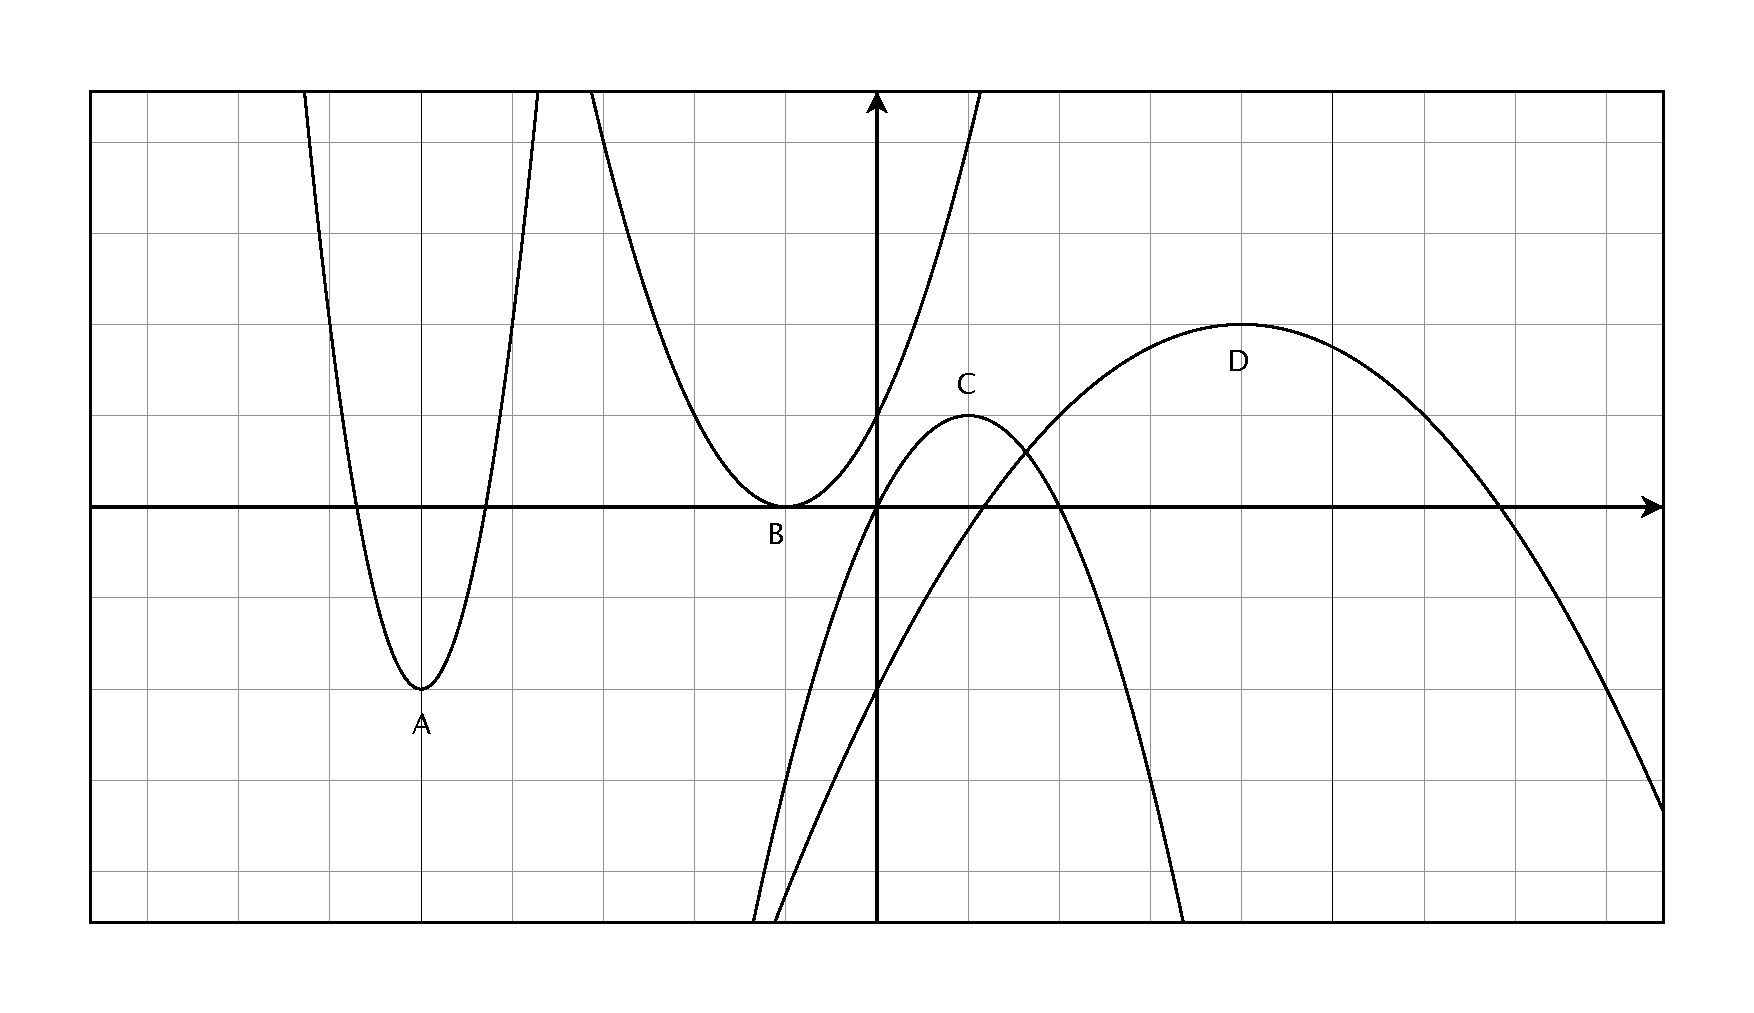
\includegraphics[scale=.3]{problem_7.eps}
%   \caption*{Problem 7}
% \end{figure}

% \begin{tabular}{cc}
% \toprule
% period & amplitude \\
% \midrule
%   $\pi$ & $2$ \\
% \bottomrule
% \end{tabular}

\title{Math 142 Notes \\ Section 5.2}

\date{\today}

\begin{document}

  \maketitle
  \tableofcontents

  \section{Sine/Cosine/Tangent}

  \subsection{Definition}

  On unit circle:
  \begin{itemize*}
    \item sine---y coordinate on unit circle
    \item cosine---x coordinate on unit circle
    \item tangent---$\sfrac{y}{x}$ ($x \neq 0$)
  \end{itemize*}

  \subsection{Examples}

  \begin{itemize*}
    \item fill in table with 0, $\pi$, $\frac{\pi}{2}$, $\frac{\pi}{6}$, $\frac{\pi}{4}$, $\frac{\pi}{3}$ (first
      quadrant only)
    \item examples in all quadrants
    \item show quadrant sign chart for all
  \end{itemize*}

  \section{Secant/Cosecant/Cotangent}
  \begin{itemize*}
    \item secant--\sfrac{1}{x} ($x \neq 0$)
    \item cosecant--\sfrac{1}{y} ($y \neq 0$)
    \item cotangent--\sfrac{x}{y} ($y \neq 0$)
  \end{itemize*}

  \subsection{Examples}

  \begin{itemize*}
    \item fill in table with 0, $\pi$, $\frac{\pi}{2}$, $\frac{\pi}{6}$, $\frac{\pi}{4}$, $\frac{\pi}{3}$ (first
      quadrant only)
    \item examples in all quadrants
    \item show quadrant sign chart for all
  \end{itemize*}

  \section{Evaluating Trigonometric Functions}

  \begin{itemize*}
    \item find reference number
    \item look up from table or memorize
    \item use appropriate sign for quadrant
  \end{itemize*}

  Do examples like $\frac{2 \pi}{3}$, $\frac{5 \pi}{4}$, $- \frac{\pi}{2}$, etc.

  \section{Domains}
  \begin{tabular}[H]{ll}
    $\sin$, $\cos$ & all real numbers \\
    $\tan$, $\sec$ & $t \neq \sfrac{\pi}{2} + n \pi$  \\
    $\cot$, $\csc$ & $t \neq n \pi$  \\
  \end{tabular}

  \section{Even/Odd}
  \subsection{Overview}
  \begin{itemize*}
    \item review even/odd definitions
    \item $\sin (-t) = -y = - \sin t$
    \item $\tan (-t) = - \sfrac{y}{x} = - \tan t$
    \item $\cos (-t) = x = \cos t$
    \item sine, cosecant, tangent, and cotangent are odd
    \item cosine and secant are even
  \end{itemize*}

  \subsection{Examples}
  \begin{itemize*}
    \item $\sin (- \sfrac{\pi}{2}) = - \sin \sfrac{\pi}{2} = \sfrac{\sqrt{2}}{2}$
    \item $\cos (- \sfrac{\pi}{2}) = \cos \sfrac{\pi}{2} = \sfrac{\sqrt{2}}{2}$

    \item $\sin x - \cos x$ (neither)
    \item $\sin x \cos x$ (odd)
    \item $x^2 \cos x$ (even)
  \end{itemize*}

  \section{Identities}

  \subsection{Fundamental Identities}
  \begin{itemize*}
    \item secant, etc. inverses of cosine, etc.
    \item $\sin^2 t + \cos^2 t = 1$
    \item $\tan^2 t + 1 = \sec^2 t$
    \item $\cot^2 t + 1 = \csc^2 t$
  \end{itemize*}

  \subsection{Applications}

  \begin{enumerate}
    \item if $\sin t = \frac{2}{5}$ and $t$ is in quadrant II, find the values of the other trigonometric functions

      \begin{align*}
        \left( \frac{4}{5} \right)^2 + \cos^2 x & = 1 \\
        \cos x                                  & = - \frac{3}{5} \\
        \\
        \tan x & = \frac{\sin x}{\cos x} \\
               & = \frac{2}{5} \times \frac{-5}{3} \\
               & = - \frac{2}{3} \\
      \end{align*}

    \item write $\sin t$ in terms of $\cos t$ where $t$ is in quadrant IV
      \begin{align*}
        \sin^2 t + \cos^2 t & = 1 \\
        \sin^2 t            & = 1 - \cos^2 t \\
        \sin t              & = - \sqrt{ 1 - \cos^2 t } \\
      \end{align*}
  \end{enumerate}

\end{document}
